\chapter{Types of Reactions}
\label{chap:reactiontypes}

There are many different types of chemical reactions that can take place. In this chapter, we will be looking at a few of the more common reaction types: acid-base and acid-carbonate reactions, redox reactions and addition, elimination and substitution reactions.

\chapterstartvideo{VPjmz}

% CHILD SECTION START

\section{Acid-base reactions}
\label{sec:reactiontypes:acid-base}

\subsection{What are acids and bases?}

In our daily lives, we encounter many examples of acids and bases. In the home, vinegar (acetic acid), lemon juice (citric acid) and tartaric acid (the main acid found in wine) are common, while hydrochloric acid, sulphuric acid and nitric acid are examples of acids that are more likely to be found in laboratories and industry. Hydrochloric acid is also found in the gastric juices in the stomach. Even fizzy drinks contain acid (carbonic acid), as do tea and wine (tannic acid)! Bases that you may know about include sodium hydroxide (caustic soda), ammonium hydroxide and ammonia. Some of these are found in household cleaning products. Acids and bases are also important commercial products in the fertiliser, plastics and petroleum refining industries. Some common acids and bases, and their chemical formulae, are shown in table \ref{tab:acids and bases}.

\begin{table}[h]
\begin{center}
\caption{Some common acids and bases and their chemical formulae}
\label{tab:acids and bases}

\begin{tabular}{|l|l||l|l|}\hline
\textbf{Acid} & \textbf{Formula} & \textbf{Base} & \textbf{Formula}\\\hline
Hydrochloric acid & HCl & Sodium hydroxide & NaOH \\\hline
Sulphuric acid & H$_{2}$SO$_{4}$ & Potassium hydroxide & KOH \\\hline
Nitric acid & HNO$_{3}$ & Sodium carbonate & Na$_{2}$CO$_{3}$\\\hline
Acetic (ethanoic) acid & CH$_{3}$COOH & Calcium hydroxide & Ca(OH)$_{2}$ \\\hline
Carbonic acid & H$_{2}$CO$_{3}$ & Magnesium hydroxide & Mg(OH)$_{2}$ \\\hline
Sulphurous acid & H$_{2}$SO$_{3}$ & Ammonia & NH$_{3}$ \\\hline
Phosphoric acid & H$_{3}$PO$_{4}$ & Sodium bicarbonate & NaHCO$_{3}$ \\\hline
\end{tabular}
\end{center}
\end{table}

Most acids share certain characteristics, and most bases also share similar characteristics. It is important to be able to have a definition for acids and bases so that they can be correctly identified in reactions.

\subsection{Defining acids and bases}

A number of definitions for acids and bases have developed over the years. One of the earliest was the \textbf{Arrhenius} definition. Arrhenius (1887) noticed that water dissociates (splits up) into hydronium (H$_{3}$O$^{+}$) and hydroxide (OH$^{-}$) ions according to the following equation:

\begin{center}
$\text{H}_{2}\text{O} \leftrightharpoons \text{H}_{3}\text{O}^{+} + \text{OH}^{-}$
\end{center}

\Tip{For more information on \textit{dissociation}, refer to Grade 10.}

Arrhenius described an acid as a compound that increases the concentration of H$_{3}$O$^{+}$ ions in solution, and a base as a compound that increases the concentration of OH$^{-}$ ions in a solution. Look at the following examples showing the dissociation of hydrochloric acid and sodium hydroxide (a base) respectively:

\begin{enumerate}
\item{
$\rm{HCl + H_{2}O \rightarrow H_{3}O^{+} + Cl^{-}}$

Hydrochloric acid in water increases the concentration of H$_{3}$O$^{+}$ ions and is therefore an \textit{acid}.}

\item{$\rm{NaOH + H_{2}O \rightarrow Na^{+} + OH^{-}}$

Sodium hydroxide in water increases the concentration of OH$^{-}$ ions and is therefore a \textit{base}.}
\end{enumerate}

However, this definition could only be used for acids and bases \textit{in water}. Since there are many reactions which do not occur in water it was important to come up with a much broader definition for acids and bases. \\

In 1923, Lowry and Bronsted took the work of Arrhenius further to develop a broader definition for acids and bases. The \textbf{Bronsted-Lowry model} defines acids and bases in terms of their ability to donate or accept protons.
\vspace{-.5cm}
\Definition{Acids and bases}{According to the Bronsted-Lowry theory of acids and bases, an \textbf{acid} is a substance that gives away protons (H$^{+}$), and is therefore called a \textbf{proton donor}. A \textbf{base} is a substance that takes up protons, and is therefore called a \textbf{proton acceptor}.}

Below are some examples:

\begin{enumerate}
\item{$\rm{HCl(g) + NH_{3}(g) \rightarrow NH_{4}^{+} + Cl^{-}}$\\

In order to decide which substance is a proton donor and which is a proton acceptor, we need to look at what happens to each reactant. The reaction can be broken down as follows:\\

$\rm{HCl \rightarrow Cl^{-} + H^{+}}$ and

$\rm{NH_{3} + H^{+} \rightarrow NH_{4}^{+}}$\\

From these reactions, it is clear that HCl is a \textit{proton donor} and is therefore an \textbf{acid}, and that NH$_{3}$ is a \textit{proton acceptor} and is therefore a \textbf{base}.
}

\item{$\rm{CH_{3}COOH + H_{2}O \rightarrow H_{3}O^{+} + CH_{3}COO^{-}}$\\

The reaction can be broken down as follows:\\

$\rm{CH_{3}COOH \rightarrow CH_{3}COO^{-} + H^{+}}$ and

$\rm{H_{2}O + H^{+} \rightarrow H_{3}O^{+}}$\\

In this reaction, CH$_{3}$COOH (acetic acid) is a proton donor and is therefore the \textbf{acid}. In this case, water acts as a \textbf{base} because it accepts a proton to form H$_{3}$O$^{+}$.
}

\item{$\rm{NH_{3} + H_{2}O \rightarrow NH_{4}^{+} + OH^{-}}$\\

The reaction can be broken down as follows:\\

$\rm{H_{2}O \rightarrow OH^{-} + H^{+}}$ and

$\rm{NH_{3} + H^{+} \rightarrow NH_{4}^{+}}$\\

In this reaction, water donates a proton and is therefore an \textbf{acid} in this reaction. Ammonia accepts the proton and is therefore the \textbf{base}. Notice that in the previous equation, water acted as a base and that in this equation it acts as an acid. Water can act as both an acid and a base depending on the reaction. This is also true of other substances. These substances are called \textbf{ampholytes} and are said to be \textbf{amphoteric}.}
\end{enumerate}

\Definition{Amphoteric}{An amphoteric substance is one that can react as either an acid or base. Examples of amphoteric substances include water, ammonia, zinc oxide and beryllium hydroxide.}


\subsection{Conjugate acid-base pairs}

Look at the reaction between hydrochloric acid and ammonia to form ammonium and chloride ions:

\begin{center}
$\text{HCl} + \text{NH}_{3} \leftrightharpoons \text{NH}_{4}^{+} + \text{Cl}^{-}$
\end{center}

Looking firstly at the \textit{forward reaction} (i.e. the reaction that proceeds from \textit{left} to \textit{right}), the changes that take place can be shown as follows:\\

$\rm{HCl \rightarrow Cl^{-} + H^{+}}$ and

$\rm{NH_{3} + H^{+} \rightarrow NH_{4}^{+}}$\\

Looking at the \textit{reverse reaction} (i.e. the reaction that proceeds from \textit{right} to \textit{left}), the changes that take place are as follows:\\

$\rm{NH_{4}^{+} \rightarrow NH_{3} + H^{+}}$ and

$\rm{Cl^{-} + H^{+} \rightarrow HCl}$\\

In the \textbf{forward reaction}, HCl is a proton donor (acid) and NH$_{3}$ is a proton acceptor (base). In the \textbf{reverse reaction}, the chloride ion is the proton acceptor (base) and NH$_{4}^{+}$ is the proton donor (acid). A \textbf{conjugate acid-base pair} is two compounds in a reaction that change into each other through the loss or gain of a proton. The conjugate acid-base pairs for the above reaction are shown below.

\begin{center}
\begin{pspicture}(-4,-2)(4,1.5)
%\psgrid[gridcolor=lightgray]
\rput(-2,0){\textbf{HCl + NH$_{3}$}}
\rput(2,0){\textbf{NH$_{4}^{+}$ + Cl$^{-}$}}
\psline[arrows=->](-0.5,0.1)(0.5,0.1)
\psline[arrows=<-](-0.5,-0.1)(0.5,-0.1)
\rput(-2.5,-0.4){acid$_{1}$}
\rput(-1.4,-0.4){base$_{2}$}
\rput(2.6,-0.4){base$_{1}$}
\rput(1.4,-0.4){acid$_{2}$}
\psline(-2.5,0.4)(-2.5,0.8)
\psline(2.6,0.4)(2.6,0.8)
\psline(-2.5,0.8)(2.6,0.8)
\rput(0,1){conjugate pair}
\psline(-1.4,-0.8)(-1.4,-1.2)
\psline(1.4,-0.8)(1.4,-1.2)
\psline(-1.4,-1.2)(1.4,-1.2)
\rput(0,-1.4){conjugate pair}
\end{pspicture}
\end{center}

The reaction between ammonia and water is another example:

\begin{center}
\begin{pspicture}(-4,-2)(4,1.5)
%\psgrid[gridcolor=lightgray]
\rput(-2,0){\textbf{H$_{2}$O + NH$_{3}$}}
\rput(2,0){\textbf{NH$_{4}^{+}$ + OH$^{-}$}}
\psline[arrows=->](-0.5,0.1)(0.5,0.1)
\psline[arrows=<-](-0.5,-0.1)(0.5,-0.1)
\rput(-2.5,-0.4){acid$_{1}$}
\rput(-1.4,-0.4){base$_{2}$}
\rput(2.6,-0.4){base$_{1}$}
\rput(1.4,-0.4){acid$_{2}$}
\psline(-2.5,0.4)(-2.5,0.8)
\psline(2.6,0.4)(2.6,0.8)
\psline(-2.5,0.8)(2.6,0.8)
\rput(0,1){conjugate pair}
\psline(-1.4,-0.8)(-1.4,-1.2)
\psline(1.4,-0.8)(1.4,-1.2)
\psline(-1.4,-1.2)(1.4,-1.2)
\rput(0,-1.4){conjugate pair}
\end{pspicture}
\end{center}

\Definition{Conjugate acid-base pair}{
The term refers to two compounds that transform into each other by the gain or loss of a proton.
}
% Khan Academy video on conjugate acids and bases: SIYAVULA-VIDEO:http://cnx.org/content/m39088/latest/#acids
\mindsetvid{Khan on acids and bases}{VPjpw} 
\pagebreak
\Exercise{Acids and bases}{
% \begin{enumerate}
% \item{In the following reactions, identify (1) the acid and the base in the reactants and (2) the salt in the product.
% \begin{enumerate}
% \item{$\rm{H_{2}SO_{4} + Ca(OH)_{2} \rightarrow CaSO_{4} + 2H_{2}O}$}
% \item{$\rm{CuO + H_{2}SO_{4} \rightarrow CuSO_{4} + H_{2}O}$}
% \item{$\rm{H_{2}O + C_{6}H_{5}OH \rightarrow H_{3}O^{+} + C_{6}H_{5}O^{-}}$}
% \item{$\rm{HBr + C_{5}H_{5}N \rightarrow (C_{5}H_{5}NH^{+})Br^{-}}$}
% \end{enumerate}}
% \item{
In each of the following reactions, label the conjugate acid-base pairs.
\begin{enumerate}
\item{$\text{H}_{2}\text{SO}_{4} + \text{H}_{2}\text{O} \leftrightharpoons \text{H}_{3}\text{O}^{+} + \text{HSO}_{4}^{-}$}
\item{$\text{NH}_{4}^{+} + \text{F}^{-} \leftrightharpoons \text{HF} + \text{NH}_{3}$}
\item{$\text{H}_{2}\text{O} + \text{CH}_{3}\text{COO}^{-} \leftrightharpoons \text{CH}_{3}\text{COOH} + \text{OH}^{-}$}
\item{$\text{H}_{2}\text{SO}_{4} + \text{Cl}^{-} \leftrightharpoons \text{HCl} + \text{HSO}_{4}^{-}$}
\end{enumerate}
% }
% \end{enumerate}
\practiceinfo

\begin{tabular}[h]{cccccc}
% (1.) 00zj 
& (1.) 00zk & 
 \end{tabular}
}

\subsection{Acid-base reactions}

When an acid and a base react, they neutralise each other to form a \textbf{salt}. If the base contains hydroxide (OH$^{-}$)  ions, then \textit{water} will also be formed. The word \textit{salt} is a general term which applies to the products of all acid-base reactions. A salt is a product that is made up of the cation from a base and the anion from an acid. When an acid reacts with a base, they \textbf{neutralise} each other. In other words, the acid becomes less acidic and the base becomes less basic. Look at the following examples:\\

\begin{enumerate}
\item{Hydrochloric acid reacts with sodium hydroxide to form sodium chloride (the salt) and water. Sodium chloride is made up of Na$^{+}$ cations from the base (NaOH) and Cl$^{-}$ anions from the acid (HCl). \\

$\rm{HCl + NaOH \rightarrow H_{2}O + NaCl}$
}

\item{Hydrogen bromide reacts with potassium hydroxide to form potassium bromide (the salt) and water. Potassium bromide is made up of K$^{+}$ cations from the base (KOH) and Br$^{-}$ anions from the acid (HBr).\\

$\rm{HBr + KOH \rightarrow H_{2}O +KBr}$
}

\item{Hydrochloric acid reacts with sodium hydrocarbonate to form sodium chloride (the salt) and hydrogen carbonate. Sodium chloride is made up of Na$^{+}$ cations from the base (NaHCO$_{3}$) and Cl$^{-}$ anions from the acid (HCl).\\

$\rm{HCl + NaHCO_{3} \rightarrow H_{2}CO_{3} + NaCl}$
}
\end{enumerate}

You should notice that in the first two examples, the base contained OH$^{-}$ ions, and therefore the products were a \textit{salt} and \textit{water}. NaCl (table salt) and KBr are both salts. In the third example, NaHCO$_{3}$ also acts as a base, despite not having OH$^{-}$ ions. A salt is still formed as one of the products, but no water is produced.\\

It is important to realise how important these neutralisation reactions are. Below are some examples:

\begin{itemize}
\item{\textbf{Domestic uses}

Calcium oxide (CaO) is put on soil that is too acid. Powdered limestone (CaCO$_{3}$) can also be used but its action is much slower and less effective. These substances can also be used on a larger scale in farming and also in rivers. }

\item{\textbf{Biological uses}

Acids in the stomach (e.g. hydrochloric acid) play an important role in helping to digest food. However, when a person has a stomach ulcer, or when there is too much acid in the stomach, these acids can cause a lot of pain. \textbf{Antacids} are taken to neutralise the acids so that they don't burn as much. Antacids are bases which neutralise the acid. Examples of antacids are aluminium hydroxide, magnesium hydroxide ('milk of magnesia') and sodium bicarbonate ('bicarbonate of soda'). Antacids can also be used to relieve heartburn.}

\item{\textbf{Industrial uses}

Alkaline calcium hydroxide (limewater) can be used to absorb harmful acidic SO$_{2}$ gas that is released from power stations and from the burning of fossil fuels.
}


\end{itemize}

\begin{IFact}{
Bee stings are acidic and have a pH between 5 and 5.5. They can be soothed by using substances such as calomine lotion, which is a mild alkali based on zinc oxide. Bicarbonate of soda can also be used. Both alkalis help to neutralise the acidic bee sting and relieve some of the itchiness!
}
\end{IFact}

\textbf{Acid-base titrations}\\

The neutralisation reaction between an acid and a base can be very useful. If an acidic solution of known concentration (a standard solution) is added to an alkaline solution until the solution is exactly neutralised (i.e. it has neither acidic nor basic properties), it is possible to calculate the exact concentration of the unknown solution. It is possible to do this because, at the exact point where the solution is neutralised, chemically equivalent amounts of acid and base have reacted with each other. This type of calculation is called \textbf{volumetric analysis}. The process where an acid solution and a basic solution are added to each other for this purpose, is called a \textbf{titration}, and the point of neutralisation is called the \textbf{end point} of the reaction. So how exactly can a titration be carried out to determine an unknown concentration? Look at the following steps to help you to understand the process.
\begin{enumerate}[label=\textbf{Step \arabic*}:]
\item A measured volume of the solution with unknown concentration is put into a flask.
\item A suitable indicator is added to this solution (bromothymol blue and phenolpthalein are common indicators).
\item A volume of the standard solution is put into a burette (a measuring device) and is slowly added to the solution in the flask, drop by drop.
\item At some point, adding one more drop will change the colour of the unknown solution. For example, if the solution is basic and bromothymol blue is being used as the indicator in the titration, the bromothymol blue would originally have coloured the solution blue. At the end point of the reaction, adding one more drop of acid will change the colour of the basic solution from blue to yellow. Yellow shows that the solution is now acidic.
\item Record the volume of standard solution that has been added up to this point.
\item Use the information you have gathered to calculate the exact concentration of the unknown solution. A worked example is shown below.
\end{enumerate}

\Tip{
When you are busy with these calculations, you will need to remember the following:

1dm$^{3} = 1$ litre $= 1~000$ ml $= 1~000$ cm$^{3}$, therefore dividing cm$^{3}$ by 1 000 will give you an answer in dm$^{3}$.\\

Some other terms and equations which will be useful to remember are shown below:
\begin{itemize}
\item{Molarity is a term used to describe the concentration of a solution, and is measured in mol.dm$^{-3}$. The symbol for molarity is M. Refer to chapter \ref{chap:quant} for more information on molarity.}
\item{Moles $=$ molarity ($\text{mol} \cdot \text{dm} ^{-3}$) $\times$ volume (dm$^{3}$)}
\item{Molarity ($\text{mol} \cdot \text{dm}^{-3}$) $=$ $\frac{\text{moles}}{\text{volume}}$}
\end{itemize}
}

\begin{wex}{Titration calculation I}{Given the equation:
\begin{center}
$\rm{NaOH + HCl \rightarrow NaCl + H_{2}O}$
\end{center}
25 cm$^{3}$ of a sodium hydroxide solution was pipetted into a conical flask and titrated with 0.2 M hydrochloric acid. Using a suitable indicator, it was found that 15 cm$^{3}$ of acid was needed to neutralise the alkali. Calculate the molarity of the sodium hydroxide.}{\westep{Write down all the information you know about the reaction, and make sure that the equation is balanced.}

NaOH: V $= 25$ cm$^{3}$

HCl: V $= 15$ cm$^{3}$; C $= 0.2$ M

The equation is already balanced.
\westep{Calculate the number of moles of HCl that react according to this equation.}

\begin{equation*}
M = \frac{n}{V}
\end{equation*}

Therefore, n(HCl) = M $\times$ V (make sure that all the units are correct!)\\

M $= 0.2$ mol$\cdot$dm$^{-3}$

V $= 15$ cm$^{3} = 0.015$ dm$^{3}$ \\

Therefore

\begin{equation*}
n(HCl) = 0.2 \times 0.015 = 0.003
\end{equation*}

There are 0.003 moles of HCl that react
\westep{Calculate the number of moles of sodium hydroxide in the reaction}

Look at the equation for the reaction. For every mole of HCl there is one mole of NaOH that is involved in the reaction. Therefore, if 0.003 moles of HCl react, we can conclude that the same quantity of NaOH is needed for the reaction. The number of moles of NaOH in the reaction is 0.003.
\westep{Calculate the molarity of the sodium hydroxide}

First convert the volume into dm$^{3}$. V $= 0.025$ dm$^{3}$. Then continue with the calculation.

\begin{equation*}
M = \dfrac{n}{V} = \frac{0.003}{0.025} = 0.12
\end{equation*}

The molarity of the NaOH solution is 0.12 mol.dm$^{3}$ \\or 0.12 M
}
\end{wex}

\begin{wex}{Titration calculation II}{4.9 g of sulphuric acid is dissolved in water and the final solution has a volume of 220 cm$^{3}$. Using titration, it was found that 20 cm$^{3}$ of this solution was able to completely neutralise 10 cm$^{3}$ of a sodium hydroxide solution. Calculate the concentration of the sodium hydroxide in mol.dm$^{-3}$.}{\westep{Write a balanced equation for the titration reaction.}

$\rm{H_{2}SO_{4} + 2NaOH \rightarrow Na_{2}SO_{4} + 2H_{2}O}$
\westep{Calculate the molarity of the sulphuric acid solution.}

$M = \dfrac{n}{V}$

V $= 220$ cm$^{3} = 0.22$ dm$^{3}$

\begin{equation*}
n = \dfrac{m}{M} = \frac{4.9 g}{98 \text{ g} \cdot \text{mol}^{-1}} = 0.05 \text{mol}
\end{equation*}

Therefore,

\begin{equation*}
M = \dfrac{0.05}{0.22} = 0.23 \text{ mol} \cdot \text{dm}^{-3}
\end{equation*}
\westep{Calculate the moles of sulphuric acid that were used in the neutralisation reaction.}

Remember that only 20 cm$^{3}$ of the sulphuric acid solution is used.\\

$M = \frac{n}{V}$, therefore $n = M \times V$

\begin{equation*}
n = 0.23 \times 0.02 = 0.0046 \text{ mol}
\end{equation*}
\westep{Calculate the number of moles of sodium hydroxide that were neutralised.}
According to the balanced chemical equation, the mole ratio of H$_{2}$SO$_{4}$ to NaOH is 1:2. Therefore, the number of moles of NaOH that are neutralised is 0.0046 $\times$ 2 = 0.0092 mol.
\westep{Calculate the concentration of the sodium hydroxide solution.}
\begin{equation*}
M = \frac{n}{V} = \frac{0.0092}{0.01} = 0.92 \text{ M}
\end{equation*}
}
\end{wex}

\subsection{Acid-carbonate reactions}

\Activity{Demonstration}{The reaction of acids with carbonates\\}{
\textbf{Apparatus and materials:}\\

Small amounts of sodium carbonate powder and calcium carbonate powder; hydrochloric acid and sulphuric acid; retort stand; two test tubes; two rubber stoppers for the test tubes; a delivery tube; lime water. The demonstration should be set up as shown below.

\begin{center}
\begin{pspicture}(-2,-0.4)(6,7)
%\psgrid[gridcolor=gray]
\def\stand{\psline[linewidth=5pt](-1.5,0)(1.5,0)\psline[linewidth=5pt](0,0)(0,5)\psframe[fillstyle=solid,fillcolor=gray,linestyle=none](-0.5,2.5)(0.5,3.5)\psline[linewidth=3pt,linecolor=gray](0.5,3)(2,3)}
\def\tube{\psarc(0,0){1.5}{0}{180}\psarc(0,0){1.75}{0}{180}\psline(1.5,0)(1.5,-1)\psline(1.75,0)(1.75,-1)}
\rput(0,-0.2){\stand}
\rput(1.5,3){\pstTubeEssais[glassType=tube,bouchon=true,niveauLiquide1=30]}
\rput(4.8,2){\pstTubeEssais[glassType=tube,bouchon=true,niveauLiquide1=60]}
\rput(3.2,5){\tube}
\rput(3.2,5){\psline(-1.5,-0.9)(-1.5,-1.25)\psline(-1.75,-0.9)(-1.75,-1.25)}
\rput(5,4){\psline(0,-0.9)(0,-1.25)\psline(-0.25,-0.9)(-0.25,-1.25)}
\uput[d](1.95,1){\parbox[l]{3.2cm}{sodium carbonate \& hydrochloric acid}}
\uput[d](4.8,0){limewater}
\uput[r](4.4,6.4){delivery tube}
\uput[l](1,5){rubber stopper}
\uput[r](5.4,4){rubber stopper}

\end{pspicture}
\end{center}


\textbf{Method:}

\begin{enumerate}
\item{Pour limewater into one of the test tubes and seal with a rubber stopper.}
\item{Carefully pour a small amount of hydrochloric acid into the other test tube.}
\item{Add a small amount of sodium carbonate to the acid and seal the test tube with the rubber stopper.}
\item{Connect the two test tubes with a delivery tube.}
\item{Observe what happens to the colour of the limewater.}
\item{Repeat the above steps, this time using sulphuric acid and calcium carbonate.}
\end{enumerate}

\textbf{Observations:}\\

The clear lime water turns milky meaning that carbon dioxide has been produced.
}

When an acid reacts with a carbonate a salt, carbon dioxide and water are formed. Look at the following examples:\\

\begin{itemize}
\item{Nitric acid reacts with sodium carbonate to form sodium nitrate, carbon dioxide and water.
\begin{center}
$\rm{2HNO_{3} + Na_{2}CO_{3} \rightarrow 2NaNO_{3} + CO_{2} + H_{2}O}$\\
\end{center}
}
\item{Sulphuric acid reacts with calcium carbonate to form calcium sulfate, carbon dioxide and water.
\begin{center}
$\rm{H_{2}SO_{4} + CaCO_{3} \rightarrow CaSO_{4} + CO_{2} + H_{2}O}$\\
\end{center}
}
\item{Hydrochloric acid reacts with calcium carbonate to form calcium chloride, carbon dioxide and water.
\begin{center}
$\rm{2HCl + CaCO_{3} \rightarrow CaCl_{2} + CO_{2} + H_{2}O}$
\end{center}
}
\end{itemize}
% Presentation on acid-base reactions: SIYAVULA-PRESENTATION:http://cnx.org/content/m39088/latest/#slidesharefigure
\Exercise{Acids and bases}{

\begin{enumerate}

\item{The compound NaHCO$_{3}$ is commonly known as baking soda. A recipe requires 1.6 g of baking soda, mixed with other ingredients, to bake a cake.
\begin{enumerate}
\item{Calculate the number of moles of NaHCO$_{3}$ used to bake the cake.}
\item{How many atoms of oxygen are there in the 1.6 g of baking soda?

During the baking process, baking soda reacts with an acid to produce carbon dioxide and water, as shown by the reaction equation below:
\begin{center}
$\rm{HCO_{3}^{-} (aq) + H^{+} (aq) \rightarrow CO_{2} (g) + H_{2}O (l)}$
\end{center}}

\item{Identify the reactant which acts as the Bronsted-Lowry base in this reaction. Give a reason for your answer.}
\item{Use the above equation to explain why the cake rises during this baking process.}
\end{enumerate}

(DoE Grade 11 Paper 2, 2007)}

\item{Label the acid-base conjugate pairs in the following equation:
\begin{center}
$\text{HCO}_{3}^{-} + \text{H}_{2}\text{O} \leftrightharpoons \text{CO}_{3}^{2-} + \text{H}_{3}\text{O}^{+}$
\end{center}
}

\item{A certain antacid tablet contains 22.0 g of baking soda (NaHCO$_{3}$). It is used to neutralise the excess hydrochloric acid in the stomach. The balanced equation for the reaction is:

\begin{center}
$\rm{NaHCO_{3} + HCl \rightarrow NaCl + H_{2}O + CO_{2}}$
\end{center}

The hydrochloric acid in the stomach has a concentration of 1.0 mol.dm$^{-3}$. Calculate the volume of the hydrochloric acid that can be neutralised by the antacid tablet.

(DoE Grade 11 Paper 2, 2007)}

\item{A learner is asked to prepare a \textit{standard solution} of the weak acid, oxalic acid (COOH)$_{2}$2H$_{2}$O for use in a titration. The volume of the solution must be 500 cm$^{3}$ and the concentration 0.2 mol.dm$^{-3}$.
\begin{enumerate}
\item{Calculate the mass of oxalic acid which the learner has to dissolve to make up the required standard solution.}
The leaner titrates this 0.2 mol.dm$^{-3}$ oxalic acid solution against a solution of sodium hydroxide. He finds that 40 cm$^{3}$ of the oxalic acid solution exactly neutralises 35 cm$^{3}$ of the sodium hydroxide solution.
\item{Calculate the concentration of the sodium hydroxide solution.}
\end{enumerate}
}

\item{A learner finds some sulphuric acid solution in a bottle labelled 'dilute sulphuric acid'. He wants to determine the concentration of the sulphuric acid solution. To do this, he decides to titrate the sulphuric acid against a standard potassium hydroxide (KOH) solution.

\begin{enumerate}
\item{What is a standard solution?}
\item{Calculate the mass of KOH which he must use to make 300 cm$^{3}$ of a 0.2 mol.dm$^{-3}$ KOH solution.}
\item{Calculate the pH of the 0.2 mol.dm$^{-3}$ KOH solution (assume standard temperature).}
\item{Write a balanced chemical equation for the reaction between H$_{2}$SO$_{4}$ and KOH.}
\item{During the titration he finds that 15 cm$^{3}$ of the KOH solution neutralises 20 cm$^{3}$ of the H$_{2}$SO$_{4}$ solution. Calculate the concentration of the H$_{2}$SO$_{4}$ solution.}
\end{enumerate}
(IEB Paper 2, 2003)
}

\end{enumerate}
\practiceinfo

\begin{tabular}[h]{cccccc}
(1.) 00zm & (2.) 00zn & (3.) 00zp & (4.) 00zq & (5.) 00zr & 
 \end{tabular}
}




% CHILD SECTION END



% CHILD SECTION START

\section{Redox reactions}
\label{sec:reactiontypes:redox}

A second type of reaction is the \textbf{redox} reaction, in which both \textbf{oxidation} and \textbf{reduction} take place.

\subsection{Oxidation and reduction}

If you look back to chapter \ref{chap:bonding}, you will remember that we discussed how, during a chemical reaction, an exchange of electrons takes place between the elements that are involved. Using \textit{oxidation numbers} is one way of tracking what is happening to these electrons in a reaction. Refer back to section \ref{sec:oxidation numbers} if you can't remember the rules that are used to give an oxidation number to an element. Below are some examples to refresh your memory before we carry on with this section.\\

\textit{Examples:}

\begin{enumerate}
\item{\textbf{CO$_{2}$}

Each oxygen atom has an oxidation number of -2. This means that the charge on \textit{two} oxygen atoms is -4. We know that the molecule of CO$_{2}$ is neutral, therefore the carbon atom must have an oxidation number of +4.}

\item{\textbf{KMnO$_{4}$}

Overall, this molecule has a neutral charge, meaning that the sum of the oxidation numbers of the elements in the molecule must equal zero. Potassium (K) has an oxidation number of +1, while oxygen (O) has an oxidation number of -2. If we exclude the atom of manganese (Mn), then the sum of the oxidation numbers equals +1+(-2x4)= -7. The atom of manganese must therefore have an oxidation number of +7 in order to make the molecule neutral.\\
}
\end{enumerate}

By looking at how the oxidation number of an element changes during a reaction, we can easily see whether that element is being \textbf{oxidised} or \textbf{reduced}.

\Definition{Oxidation and reduction}{Oxidation is the \textit{loss} of an electron by a molecule, atom or ion. Reduction is the \textit{gain} of an electron by a molecule, atom or ion.}


\textit{Example:}


\begin{center}
$\rm{Mg + Cl_{2} \rightarrow MgCl_{2}}$
\end{center}

As a \textit{reactant}, magnesium has an oxidation number of zero, but as part of the \textit{product} magnesium chloride, the element has an oxidation number of +2. Magnesium has \textit{lost} two electrons and has therefore been \textit{oxidised}. This can be written as a \textbf{half-reaction}. The half-reaction for this change is:

\begin{center}
$\rm{Mg \rightarrow Mg^{2+} + 2e^{-}}$
\end{center}

As a \textit{reactant}, chlorine has an oxidation number of zero, but as part of the \textit{product} magnesium chloride, the element has an oxidation number of -1. Each chlorine atom has \textit{gained} an electron and the element has therefore been \textit{reduced}. The half-reaction for this change is:

\begin{center}
$\rm{Cl_{2} + 2e^{-} \rightarrow 2Cl^{-}}$
\end{center}

\Tip{Oxidation and reduction made easy!\\
An easy way to think about oxidation and reduction is to remember:\\
'OILRIG' - \textbf{O}xidation \textbf{I}s \textbf{L}oss of electrons, \textbf{R}eduction \textbf{I}s \textbf{G}ain of electrons.}

\Definition{Half-reaction}{
A half reaction is either the oxidation or reduction reaction part of a redox reaction. A half reaction is obtained by considering the change in oxidation states of the individual substances that are involved in the redox reaction.
}

An element that is \textbf{oxidised} is called a \textbf{reducing agent}, while an element that is \textbf{reduced} is called an \textbf{oxidising agent}.

\subsection{Redox reactions}

\Definition{Redox reaction}{A redox reaction is one involving oxidation and reduction, where there is always a change in the oxidation numbers of the elements involved.}

\begin{g_experiment}{Redox reactions\\}{
\textbf{Materials: } A few granules of zinc; 15 ml copper (II) sulphate solution (blue colour), glass beaker.\\

\begin{center}
\begin{pspicture}(-4,-1.5)(4,2.5)
\rput(-2,0){
\rput(2,0){\filledbeaker}
\def\chip{\psframe[fillstyle=solid,fillcolor=lightgray](0,0)(0.1,0.1)}
\rput(0.2,0.01){\chip}
\rput{45}(0.1,0.05){\chip}
\rput{30}(0.3,0.05){\chip}
\rput{60}(0.2,0.2){\chip}
\rput{90}(0.35,0.2){\chip}
\rput{96}(0.15,0.2){\chip}
\rput{120}(0.3,0.1){\chip}
\rput(2.8,-0.5){copper sulphate}
\rput(2.8,-0.8){solution}
\rput(0.2,-0.5){zinc granules}
}
\end{pspicture}
\end{center}


\textbf{Method: } Add the zinc granules to the copper sulfate solution and observe what happens. What happens to the zinc granules? What happens to the colour of the solution?\\
\textbf{Results: }
\begin{itemize}
\item{Zinc becomes covered in a layer that looks like copper.}
\item{The blue copper sulphate solution becomes clearer.}
\end{itemize}

Cu$^{2+}$ ions from the CuSO$_{4}$ solution are \textbf{reduced} to form copper metal. This is what you saw on the zinc crystals. The reduction of the copper ions (in other words, their removal from the copper sulphate solution), also explains the change in colour of the solution (copper ions in solution are blue). The equation for this reaction is:
\begin{center}
$\rm{Cu^{2+} + 2e^{-} \rightarrow Cu}$
\end{center}

Zinc is \textbf{oxidised} to form Zn$^{2+}$ ions which are clear in the solution. The equation for this reaction is:
\begin{center}
$\rm{Zn \rightarrow Zn^{2+} + 2e^{-}}$
\end{center}

The overall reaction is:
\begin{center}
$\rm{Cu^{2+}(aq) + Zn(s) \rightarrow Cu(s) + Zn^{2+}(aq)}$
\end{center}

\textbf{Conclusion: } A redox reaction has taken place. Cu$^{2+}$ ions are reduced and the zinc is oxidised.
}
\end{g_experiment}

Below are some further examples of redox reactions:

\begin{itemize}
\item{$\rm{H_{2} + F_{2} \rightarrow 2HF}$ can be re-written as two half-reactions:
\begin{center}
$\rm{H_{2} \rightarrow 2H^{+} + 2e^{-}}$ (oxidation) and

$\rm{F_{2} + 2e^{-} \rightarrow 2F^{-}}$ (reduction)
\end{center}
}

\item{$\rm{Cl_{2} + 2KI \rightarrow 2KCl + I_{2}}$ or $\rm{Cl_{2} + 2I^{-} \rightarrow 2Cl^{-} + I_{2}}$, can be written as two half-reactions:
\begin{center}
$\rm{Cl_{2} + 2e^{-} \rightarrow 2Cl^{-}}$ (reduction) and

$\rm{2I^{-} \rightarrow I_{2} + 2e^{-}}$ (oxidation)
\end{center}
}
\end{itemize}

In Grade 12, you will go on to look at electrochemical reactions, and the role that electron transfer plays in this type of reaction.\\
% Khan Academy video on oxidation states: SIYAVULA-VIDEO:http://cnx.org/content/m39092/latest/#redox-1
\mindsetvid{Khan on oxidation states}{VPjql}
% Presentation on redox reactions: SIYAVULA-PRESENTATION:http://cnx.org/content/m39092/latest/#slidesharefigure1
\Exercise{Redox Reactions\\}{
\begin{enumerate}

\item{Look at the following reaction:
\begin{center}
$2\text{H}_{2}\text{O}_{2} (\ell) \rightarrow 2\text{H}_{2}\text{O} (\ell) + \text{O}_{2} \text{(g)}$
\end{center}

\begin{enumerate}
\item{What is the oxidation number of the oxygen atom in each of the following compounds?}
\begin{enumerate}
\item{H$_{2}$O$_{2}$}
\item{H$_{2}$O}
\item{O$_{2}$}
\end{enumerate}
\item{Does the hydrogen peroxide (H$_{2}$O$_{2}$) act as an oxidising agent or a reducing agent or both, in the above reaction? Give a reason for your answer.}
\end{enumerate}
}


\item{
Consider the following chemical equations:

1. $\rm{Fe (s) \rightarrow Fe^{2+} (aq) + 2e^{-}}$

2. $4\text{H}^{+} \text{ (aq)} + \text{O}_{2} \text{ (g)} + 4e^{-} \rightarrow 2\text{H}_{2}\text{O} (\ell) $\\

Which one of the following statements is correct?

\begin{enumerate}
\item{Fe is oxidised and H$^{+}$ is reduced}
\item{Fe is reduced and O$_{2}$ is oxidised}
\item{Fe is oxidised and O$_{2}$ is reduced}
\item{Fe is reduced and H$^{+}$ is oxidised}
\end{enumerate}
}
(DoE Grade 11 Paper 2, 2007)

\item{Which one of the following reactions is a redox reaction?}
\begin{enumerate}
\item{$\rm{HCl + NaOH \rightarrow NaCl + H_{2}O}$}
\item{$\rm{AgNO_{3} + NaI \rightarrow AgI + NaNO_{3}}$}
\item{$\rm{2FeCl_{3} + 2H_{2}O + SO_{2} \rightarrow H_{2}SO_{4} + 2HCl + 2FeCl_{2}}$}
\item{$\rm{BaCl_{2} + MgSO_{4} \rightarrow MgCl_{2} + BaSO_{4}}$}
\end{enumerate}

\end{enumerate}
\practiceinfo

\begin{tabular}[h]{cccccc}
(1.) 00zs & (2.) 00zt & (3.) 00zu & 
 \end{tabular}
}


% CHILD SECTION END



% CHILD SECTION START

\section{Addition, substitution and elimination reactions}

\subsection{Addition reactions}

An addition reaction occurs when two or more reactants combine to form a final product. This product will contain \textit{all} the atoms that were present in the reactants. The following is a general equation for this type of reaction:

\begin{equation*}
A + B \rightarrow C
\end{equation*}

Notice that C is the final product with no A or B remaining as a residue.\\

The following are some examples.

\begin{enumerate}
\item{The reaction between \textbf{ethene} and \textbf{bromine} to form 1,2-dibromoethane (figure \ref{fig:types:addition}).

\begin{center}
$\rm{C_{2}H_{4} + Br_{2} \rightarrow C_{2}H_{4}Br_{2}}$
\end{center}
}

\begin{figure}[!h]
\begin{center}
\begin{pspicture}(0,-2)(13,2)
%\psgrid[gridcolor=lightgray]
\rput(1,1){\textbf{H}}
\rput(1,-1){\textbf{H}}
\rput(2,0){\textbf{C}}
\psline(1.8,0.3)(1.2,0.7)
\psline(1.8,-0.3)(1.2,-0.7)
\psline(2.2,0.05)(2.8,0.05)
\psline(2.2,-0.05)(2.8,-0.05)
\rput(3,0){\textbf{C}}
\psline(3.2,0.3)(3.8,0.7)
\psline(3.2,-0.3)(3.8,-0.7)
\rput(4,1){\textbf{H}}
\rput(4,-1){\textbf{H}}
\rput(5,0){\textbf{+}}
\rput(6,0){\textbf{Br}}
\psline(6.3,0)(6.7,0)
\rput(7,0){\textbf{Br}}
\psline[arrows=->](7.5,0)(8.5,0)
\rput(13,0){
\rput(-4,0){\textbf{H}}
\psline(-3.8,0)(-3.2,0)
\rput(-3,0){\textbf{C}}
\psline(-3,0.2)(-3,0.8)
\rput(-3,1){\textbf{H}}
\psline(-3,-0.2)(-3,-0.8)
\rput(-3,-1){\textbf{Br}}
\rput(1,0){
\psline(-3.8,0)(-3.2,0)
\rput(-3,0){\textbf{C}}
\psline(-3,0.2)(-3,0.8)
\rput(-3,1){\textbf{H}}
\psline(-3,-0.2)(-3,-0.8)
\rput(-3,-1){\textbf{Br}}
}}
\psline(11.2,0)(11.8,0)
\rput(12,0){\textbf{H}}
\end{pspicture}
\end{center}
\caption{The reaction between ethene and bromine is an example of an addition reaction}
\label{fig:types:addition}
\end{figure}
\vspace{.5cm}
\item{\textbf{Polymerisation reactions}

In industry, making polymers is very important. A polymer is made up of lots of smaller units called \textit{monomers}. When these monomers are added together, they form a polymer. Examples of polymers are polyvinylchloride (PVC) and polystyrene. PVC is often used to make piping, while polystyrene is an important packaging and insulating material. Polystyrene is made up of lots of styrene monomers which are joined through addition reactions (figure \ref{fig:orgmac:polystyrene}). 'Polymerisation' refers to the addition reactions that eventually help to form the polystyrene polymer.

\begin{figure}[h]
\begin{center}
\scalebox{.8} % Change this value to rescale the drawing.
{
\begin{pspicture}(0,-2.11)(14.273173,2.13)
\psline[linewidth=0.028222222cm](0.85411114,-0.1184375)(0.85411114,0.6815625)
\usefont{T1}{ptm}{m}{n}
\rput(0.96832985,0.8615625){\textbf{CH}}
\usefont{T1}{ptm}{m}{n}
\rput(1.7883298,1.8815625){\textbf{CH$_{2}$}}
\psline[linewidth=0.028222222cm,arrowsize=0.05291667cm 2.0,arrowlength=1.4,arrowinset=0.4]{->}(2.3741112,-0.9384375)(4.374111,-0.9384375)
\usefont{T1}{ptm}{m}{n}
\rput(3.3739548,-0.7384375){polymerisation}
\usefont{T1}{ptm}{m}{n}
\rput(6.34833,0.8615625){\textbf{CH}}
\psline[linewidth=0.028222222cm](6.424111,1.0615625)(7.22,1.75)
\usefont{T1}{ptm}{m}{n}
\rput(7.60833,1.8815625){\textbf{CH$_{2}$}}
\usefont{T1}{ptm}{m}{n}
\rput(8.84833,0.8615625){\textbf{CH}}
\usefont{T1}{ptm}{m}{n}
\rput(11.34833,0.8615625){\textbf{CH}}
\psline[linewidth=0.028222222cm](7.88,1.71)(8.674111,1.0615625)
\usefont{T1}{ptm}{m}{n}
\rput(13.861455,-0.9384375){etc}
\pspolygon[linewidth=0.04](0.84,-2.07)(0.0,-1.518)(0.0,-0.57336)(0.86,-0.09)(1.74,-0.59)(1.74,-1.53)
\pscircle[linewidth=0.04,dimen=outer](0.88,-1.07){0.72}
\psline[linewidth=0.028222222cm](6.394111,-0.0984375)(6.394111,0.7015625)
\pspolygon[linewidth=0.04](6.36,-2.05)(5.52,-1.498)(5.52,-0.55336)(6.38,-0.07)(7.26,-0.57)(7.26,-1.51)
\pscircle[linewidth=0.04,dimen=outer](6.4,-1.05){0.72}
\psline[linewidth=0.028222222cm](8.874111,-0.0984375)(8.874111,0.7015625)
\pspolygon[linewidth=0.04](8.84,-2.07)(8.0,-1.518)(8.0,-0.57336)(8.86,-0.09)(9.74,-0.59)(9.74,-1.53)
\pscircle[linewidth=0.04,dimen=outer](8.88,-1.07){0.72}
\psline[linewidth=0.028222222cm](11.374111,-0.1184375)(11.374111,0.6815625)
\pspolygon[linewidth=0.04](11.36,-2.09)(10.52,-1.538)(10.52,-0.59336)(11.38,-0.11)(12.26,-0.61)(12.26,-1.55)
\pscircle[linewidth=0.04,dimen=outer](11.4,-1.09){0.72}
\psline[linewidth=0.028222222cm](9.124111,1.0815625)(9.92,1.77)
\usefont{T1}{ptm}{m}{n}
\rput(10.22833,1.9415625){\textbf{CH$_{2}$}}
\psline[linewidth=0.028222222cm](10.58,1.73)(11.374111,1.0815625)
\psline[linewidth=0.028222222cm](11.724112,1.1015625)(12.52,1.79)
\usefont{T1}{ptm}{m}{n}
\rput(12.82833,1.9215626){\textbf{CH$_{2}$}}
\psline[linewidth=0.028222222cm](13.02,1.75)(13.814111,1.1015625)
\psline[linewidth=0.04cm,doubleline=true,doublesep=0.06](0.96,1.03)(1.52,1.73)
\end{pspicture} 
}

\end{center}
\caption{The polymerisation of a styrene monomer to form a polystyrene polymer}
\label{fig:orgmac:polystyrene}
\end{figure}
}

\item{The \textbf{hydrogenation} of vegetable oils to form margarine is another example of an addition reaction. Hydrogenation involves adding hydrogen (H$_{2}$) to an alkene. An alkene is an organic compound composed of carbon and hydrogen. It contains a double bond between two of the carbon atoms. During hydrogenation, this double bond is broken, and more hydrogen atoms are added to the molecule. The reaction that takes place is shown below. Note that the 'R' represents any side-chain or the rest of the molecule. A side-chain is simply any combination of atoms that are attached to the central part of the molecule.

\begin{center}
$\rm{RCHCH_{2} + H_{2} \rightarrow RCH_{2}CH_{3}}$
\end{center}
}

\item{The production of ethanol (an alcohol) from ethene. Ethanol (CH$_{3}$CH$_{2}$OH) can be made from alkenes such as ethene (C$_{2}$H$_{4}$), through a hydration reaction like the one below. A hydration reaction is one where water is added to the reactants.

\begin{equation*}
\text{C}_{2}\text{H}_{4} + \text{H}_{2}\text{O}  \rightarrow \text{CH}_{3}\text{CH}_{2}\text{OH}
\end{equation*}

A catalyst is needed for this reaction to take place. The catalyst that is most commonly used is phosphoric acid.
}

\end{enumerate}


\subsection{Elimination reactions}

An elimination reaction occurs when a reactant is broken up into two products. The general form of the equation is as follows:

\begin{equation*}
A \rightarrow B + C
\end{equation*}

The examples below will help to explain this:

\begin{enumerate}
\item{
The \textbf{dehydration of an alcohol} is one example. Two hydrogen atoms and one oxygen atom are eliminated and a molecule of water is formed as a product in the reaction, along with an alkene. \\

\begin{center}
\scalebox{.8} % Change this value to rescale the drawing.
{
\begin{pspicture}(0,-1.2039063)(13.308437,1.2039063)
\usefont{T1}{ptm}{m}{n}
\rput(0.74359375,0.02390625){\textbf{H}}
\psline[linewidth=0.028222222cm](0.969375,0.02390625)(1.569375,0.02390625)
\usefont{T1}{ptm}{m}{n}
\rput(1.7435937,0.02390625){\textbf{C}}
\psline[linewidth=0.028222222cm](1.769375,0.22390625)(1.769375,0.82390624)
\usefont{T1}{ptm}{m}{n}
\rput(1.7435937,1.0239062){\textbf{H}}
\psline[linewidth=0.028222222cm](1.769375,-0.17609376)(1.769375,-0.7760937)
\usefont{T1}{ptm}{m}{n}
\rput(1.7435937,-0.97609377){\textbf{H}}
\psline[linewidth=0.028222222cm](1.969375,0.02390625)(2.569375,0.02390625)
\usefont{T1}{ptm}{m}{n}
\rput(2.7435937,0.02390625){\textbf{C}}
\psline[linewidth=0.028222222cm](2.769375,0.22390625)(2.769375,0.82390624)
\usefont{T1}{ptm}{m}{n}
\rput(2.7435937,1.0239062){\textbf{H}}
\psline[linewidth=0.028222222cm](2.769375,-0.17609376)(2.769375,-0.7760937)
\usefont{T1}{ptm}{m}{n}
\rput(2.7435937,-0.97609377){\textbf{OH}}
\psline[linewidth=0.028222222cm](2.969375,0.02390625)(3.569375,0.02390625)
\usefont{T1}{ptm}{m}{n}
\rput(3.7435937,0.02390625){\textbf{H}}
\psline[linewidth=0.028222222cm,arrowsize=0.05291667cm 2.0,arrowlength=1.4,arrowinset=0.4]{->}(4.169375,0.02390625)(5.369375,0.02390625)
\usefont{T1}{ptm}{m}{n}
\rput(5.7435937,1.0239062){\textbf{H}}
\usefont{T1}{ptm}{m}{n}
\rput(5.7435937,-0.97609377){\textbf{H}}
\usefont{T1}{ptm}{m}{n}
\rput(6.7435937,0.02390625){\textbf{C}}
\psline[linewidth=0.028222222cm](6.569375,0.32390624)(5.969375,0.7239063)
\psline[linewidth=0.028222222cm](6.569375,-0.27609375)(5.969375,-0.67609376)
\psline[linewidth=0.028222222cm](6.969375,0.07390625)(7.569375,0.07390625)
\psline[linewidth=0.028222222cm](6.969375,-0.02609375)(7.569375,-0.02609375)
\usefont{T1}{ptm}{m}{n}
\rput(7.7435937,0.02390625){\textbf{C}}
\psline[linewidth=0.028222222cm](7.969375,0.32390624)(8.569375,0.7239063)
\psline[linewidth=0.028222222cm](7.969375,-0.27609375)(8.569375,-0.67609376)
\usefont{T1}{ptm}{m}{n}
\rput(8.743594,1.0239062){\textbf{H}}
\usefont{T1}{ptm}{m}{n}
\rput(8.743594,-0.97609377){\textbf{H}}
\usefont{T1}{ptm}{m}{n}
\rput(9.743594,0.02390625){\textbf{+}}
\usefont{T1}{ptm}{m}{n}
\rput(11.003593,-0.51609373){\textbf{H}}
\psline[linewidth=0.028222222cm](11.2,-0.31609374)(11.689375,0.12390625)
\usefont{T1}{ptm}{m}{n}
\rput(11.823594,0.22390625){\textbf{O}}
\psline[linewidth=0.028222222cm](11.98,0.12390625)(12.4,-0.33609375)
\usefont{T1}{ptm}{m}{n}
\rput(12.523594,-0.55609375){\textbf{H}}
\end{pspicture} 
}
\end{center}


\begin{center}
$\rm{CH_{3}CH_{2}OH \rightarrow CH_{2}CH_{2} + H_{2}O}$
\end{center}

}

\item{The elimination of \textbf{potassium bromide from a bromoalkane}.

\begin{center}
$\rm{CH_{3}CH_{2}Br + KOH \rightarrow CH_{2}CH_{2} + KBr + H_{2}O}$
\end{center}

\begin{center}
\scalebox{.8} % Change this value to rescale the drawing.
{
\begin{pspicture}(0,-1.2039063)(13.07,1.2039063)
\usefont{T1}{ptm}{m}{n}
\rput(5.987344,1.0239062){\textbf{H}}
\usefont{T1}{ptm}{m}{n}
\rput(5.987344,-0.97609377){\textbf{H}}
\usefont{T1}{ptm}{m}{n}
\rput(6.987344,0.02390625){\textbf{C}}
\psline[linewidth=0.028222222cm](6.813125,0.32390624)(6.213125,0.7239063)
\psline[linewidth=0.028222222cm](6.813125,-0.27609375)(6.213125,-0.67609376)
\psline[linewidth=0.028222222cm](7.213125,0.07390625)(7.813125,0.07390625)
\psline[linewidth=0.028222222cm](7.213125,-0.02609375)(7.813125,-0.02609375)
\usefont{T1}{ptm}{m}{n}
\rput(7.987344,0.02390625){\textbf{C}}
\psline[linewidth=0.028222222cm](8.213125,0.32390624)(8.813125,0.7239063)
\psline[linewidth=0.028222222cm](8.213125,-0.27609375)(8.813125,-0.67609376)
\usefont{T1}{ptm}{m}{n}
\rput(8.987344,1.0239062){\textbf{H}}
\usefont{T1}{ptm}{m}{n}
\rput(8.987344,-0.97609377){\textbf{H}}
\usefont{T1}{ptm}{m}{n}
\rput(0.116875,0.00390625){H}
\psline[linewidth=0.028222222cm](0.42375,0.00390625)(0.82375,0.00390625)
\usefont{T1}{ptm}{m}{n}
\rput(1.1109375,0.00390625){C}
\psline[linewidth=0.028222222cm](1.12375,0.30390626)(1.12375,0.70390624)
\usefont{T1}{ptm}{m}{n}
\rput(1.116875,1.0039062){H}
\psline[linewidth=0.028222222cm](1.12375,-0.29609376)(1.12375,-0.69609374)
\usefont{T1}{ptm}{m}{n}
\rput(1.116875,-0.99609375){H}
\psline[linewidth=0.028222222cm](1.42375,0.00390625)(1.82375,0.00390625)
\usefont{T1}{ptm}{m}{n}
\rput(2.1109376,0.00390625){C}
\psline[linewidth=0.028222222cm](2.12375,0.30390626)(2.12375,0.70390624)
\usefont{T1}{ptm}{m}{n}
\rput(2.121875,1.0039062){Br}
\psline[linewidth=0.028222222cm](2.12375,-0.29609376)(2.12375,-0.69609374)
\usefont{T1}{ptm}{m}{n}
\rput(2.116875,-0.99609375){H}
\psline[linewidth=0.028222222cm](2.42375,0.00390625)(2.82375,0.00390625)
\usefont{T1}{ptm}{m}{n}
\rput(3.116875,0.00390625){H}
\usefont{T1}{ptm}{m}{n}
\rput(3.4184375,0.00390625){+}
\usefont{T1}{ptm}{m}{n}
\rput(4.117031,0.00390625){KOH}
\psline[linewidth=0.028222222cm,arrowsize=0.05291667cm 2.0,arrowlength=1.4,arrowinset=0.4]{->}(4.62375,0.00390625)(5.62375,0.00390625)
\usefont{T1}{ptm}{m}{n}
\rput(10.018437,0.04390625){+}
\usefont{T1}{ptm}{m}{n}
\rput(10.741875,0.02390625){KBr}
\usefont{T1}{ptm}{m}{n}
\rput(11.538438,0.02390625){+}
\usefont{T1}{ptm}{m}{n}
\rput(12.23375,0.02390625){H$_{2}$O}
\end{pspicture} 
}
\end{center}




}

\item{Ethane cracking is an important industrial process used by SASOL and other petrochemical industries. Hydrogen is eliminated from ethane (C$_{2}$H$_{6}$) to produce an alkene called ethene (C$_{2}$H$_{4}$). Ethene is then used to produce other products such as polyethylene. You will learn more about these compounds in Grade 12. The equation for the cracking of ethane looks like this:

\begin{center}
$\rm{C_{2}H_{6} \rightarrow C_{2}H_{4} + H_{2}}$
\end{center}
}

\end{enumerate}

\subsection{Substitution reactions}

A substitution reaction occurs when an exchange of elements in the reactants takes place. The initial reactants are transformed or 'swopped around' to give a final product. A simple example of a reaction like this is shown below:

\begin{equation*}
\text{AB} + \text{CD} \rightarrow \text{AC} + \text{BD}
\end{equation*}

Some simple examples of substitution reactions are shown below:

\begin{equation*}
\text{CH}_{4} + \text{Cl}_{2} \rightarrow \text{CH}_{3}\text{Cl} + \text{HCl}
\end{equation*}

In this example, a chlorine atom and a hydrogen atom are exchanged to create a new product.

\begin{equation*}
\text{Cu(H}_{2}\text{O)}_{4}^{2+} + 4\text{Cl}^{-} \rightleftharpoons \text{Cu(Cl)}_{4}^{2-} + 4\text{H}_{2}\text{O}
\end{equation*}

In this example, four waters and four chlorines are exchanged to create a new product.

\Exercise{Addition, substitution and elimination reactions\\}{
\begin{enumerate}

\item{Refer to the diagram below and then answer the questions that follow:}
\begin{center}
\scalebox{.8} % Change this value to rescale the drawing.
{
\begin{pspicture}(0,-1.2039063)(13.07,1.2039063)
\usefont{T1}{ptm}{m}{n}
\rput(5.987344,1.0239062){\textbf{H}}
\usefont{T1}{ptm}{m}{n}
\rput(5.987344,-0.97609377){\textbf{H}}
\usefont{T1}{ptm}{m}{n}
\rput(6.987344,0.02390625){\textbf{C}}
\psline[linewidth=0.028222222cm](6.813125,0.32390624)(6.213125,0.7239063)
\psline[linewidth=0.028222222cm](6.813125,-0.27609375)(6.213125,-0.67609376)
\psline[linewidth=0.028222222cm](7.213125,0.07390625)(7.813125,0.07390625)
\psline[linewidth=0.028222222cm](7.213125,-0.02609375)(7.813125,-0.02609375)
\usefont{T1}{ptm}{m}{n}
\rput(7.987344,0.02390625){\textbf{C}}
\psline[linewidth=0.028222222cm](8.213125,0.32390624)(8.813125,0.7239063)
\psline[linewidth=0.028222222cm](8.213125,-0.27609375)(8.813125,-0.67609376)
\usefont{T1}{ptm}{m}{n}
\rput(8.987344,1.0239062){\textbf{H}}
\usefont{T1}{ptm}{m}{n}
\rput(8.987344,-0.97609377){\textbf{H}}
\usefont{T1}{ptm}{m}{n}
\rput(0.116875,0.00390625){H}
\psline[linewidth=0.028222222cm](0.42375,0.00390625)(0.82375,0.00390625)
\usefont{T1}{ptm}{m}{n}
\rput(1.1109375,0.00390625){C}
\psline[linewidth=0.028222222cm](1.12375,0.30390626)(1.12375,0.70390624)
\usefont{T1}{ptm}{m}{n}
\rput(1.116875,1.0039062){H}
\psline[linewidth=0.028222222cm](1.12375,-0.29609376)(1.12375,-0.69609374)
\usefont{T1}{ptm}{m}{n}
\rput(1.116875,-0.99609375){H}
\psline[linewidth=0.028222222cm](1.42375,0.00390625)(1.82375,0.00390625)
\usefont{T1}{ptm}{m}{n}
\rput(2.1109376,0.00390625){C}
\psline[linewidth=0.028222222cm](2.12375,0.30390626)(2.12375,0.70390624)
\usefont{T1}{ptm}{m}{n}
\rput(2.1034374,1.0039062){Cl}
\psline[linewidth=0.028222222cm](2.12375,-0.29609376)(2.12375,-0.69609374)
\usefont{T1}{ptm}{m}{n}
\rput(2.116875,-0.99609375){H}
\psline[linewidth=0.028222222cm](2.42375,0.00390625)(2.82375,0.00390625)
\usefont{T1}{ptm}{m}{n}
\rput(3.116875,0.00390625){H}
\usefont{T1}{ptm}{m}{n}
\rput(3.4184375,0.00390625){+}
\usefont{T1}{ptm}{m}{n}
\rput(4.117031,0.00390625){KOH}
\psline[linewidth=0.028222222cm,arrowsize=0.05291667cm 2.0,arrowlength=1.4,arrowinset=0.4]{->}(4.62375,0.00390625)(5.62375,0.00390625)
\usefont{T1}{ptm}{m}{n}
\rput(10.018437,0.04390625){+}
\usefont{T1}{ptm}{m}{n}
\rput(10.727032,0.02390625){KCl}
\usefont{T1}{ptm}{m}{n}
\rput(11.538438,0.02390625){+}
\usefont{T1}{ptm}{m}{n}
\rput(12.23375,0.02390625){H$_{2}$O}
\end{pspicture} 
}
\end{center}

% \begin{center}
% 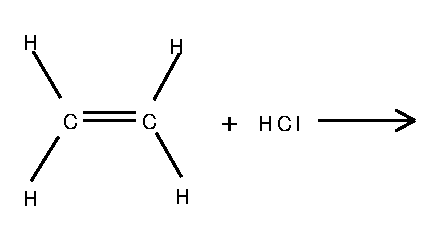
\includegraphics{../addition_rxn.eps}
% % addition_rxn.eps: 0x0 pixel, 300dpi, 0.00x0.00 cm, bb=7 8 203 104
% \end{center}


\begin{enumerate}
\item{Is this reaction an example of substitution, elimination or addition?}
\item{Give a reason for your answer above.}
\end{enumerate}

\item{The following diagram shows the reactants in an addition reaction.}

\begin{center}
\scalebox{.8} % Change this value to rescale the drawing.
{
\begin{pspicture}(0,-1.2039063)(7.314111,1.2039063)
\usefont{T1}{ptm}{m}{n}
\rput(0.74359375,1.0239062){\textbf{H}}
\usefont{T1}{ptm}{m}{n}
\rput(0.74359375,-0.97609377){\textbf{H}}
\usefont{T1}{ptm}{m}{n}
\rput(1.7435937,0.02390625){\textbf{C}}
\psline[linewidth=0.028222222cm](1.569375,0.32390624)(0.969375,0.7239063)
\psline[linewidth=0.028222222cm](1.569375,-0.27609375)(0.969375,-0.67609376)
\psline[linewidth=0.028222222cm](1.969375,0.07390625)(2.569375,0.07390625)
\psline[linewidth=0.028222222cm](1.969375,-0.02609375)(2.569375,-0.02609375)
\usefont{T1}{ptm}{m}{n}
\rput(2.7435937,0.02390625){\textbf{C}}
\psline[linewidth=0.028222222cm](2.969375,0.32390624)(3.569375,0.7239063)
\psline[linewidth=0.028222222cm](2.969375,-0.27609375)(3.569375,-0.67609376)
\usefont{T1}{ptm}{m}{n}
\rput(3.7435937,1.0239062){\textbf{H}}
\usefont{T1}{ptm}{m}{n}
\rput(3.7435937,-0.97609377){\textbf{H}}
\psline[linewidth=0.028222222cm,arrowsize=0.05291667cm 2.0,arrowlength=1.4,arrowinset=0.4]{->}(6.3,0.02390625)(7.3,0.02390625)
\usefont{T1}{ptm}{m}{n}
\rput(4.7746873,0.04390625){+}
\usefont{T1}{ptm}{m}{n}
\rput(5.483125,0.02390625){HCl}
\end{pspicture} 
}
\end{center}

\begin{enumerate}
\item{Draw the final product in this reaction.}
\item{What is the chemical formula of the product?}
\end{enumerate}

\item{The following reaction takes place:}

\begin{center}
\scalebox{.8} % Change this value to rescale the drawing.
{
\begin{pspicture}(0,-1.2039062)(11.706875,1.2039062)
\usefont{T1}{ptm}{m}{n}
\rput(5.9684377,1.0239062){\textbf{H}}
\usefont{T1}{ptm}{m}{n}
\rput(5.9684377,-0.9760937){\textbf{H}}
\usefont{T1}{ptm}{m}{n}
\rput(6.9684377,0.023906285){\textbf{C}}
\psline[linewidth=0.028222222cm](6.82,0.32390627)(6.22,0.72390634)
\psline[linewidth=0.028222222cm](6.82,-0.27609372)(6.22,-0.6760937)
\psline[linewidth=0.028222222cm](7.22,0.07390629)(7.82,0.07390629)
\psline[linewidth=0.028222222cm](7.22,-0.026093716)(7.82,-0.026093716)
\usefont{T1}{ptm}{m}{n}
\rput(7.9684377,0.023906285){\textbf{C}}
\psline[linewidth=0.028222222cm](8.22,0.32390627)(8.82,0.72390634)
\psline[linewidth=0.028222222cm](8.22,-0.27609372)(8.82,-0.6760937)
\usefont{T1}{ptm}{m}{n}
\rput(8.968438,1.0239062){\textbf{H}}
\usefont{T1}{ptm}{m}{n}
\rput(8.968438,-0.9760937){\textbf{H}}
\usefont{T1}{ptm}{m}{n}
\rput(0.116875,0.003906285){H}
\psline[linewidth=0.028222222cm](0.430625,0.003906285)(0.830625,0.003906285)
\usefont{T1}{ptm}{m}{n}
\rput(1.105,0.003906285){C}
\psline[linewidth=0.028222222cm](1.130625,0.3039063)(1.130625,0.7039063)
\usefont{T1}{ptm}{m}{n}
\rput(1.116875,1.0039062){H}
\psline[linewidth=0.028222222cm](1.130625,-0.29609373)(1.130625,-0.6960937)
\usefont{T1}{ptm}{m}{n}
\rput(1.116875,-0.9960937){H}
\psline[linewidth=0.028222222cm](1.430625,0.003906285)(1.830625,0.003906285)
\usefont{T1}{ptm}{m}{n}
\rput(2.105,0.003906285){C}
\psline[linewidth=0.028222222cm](2.130625,0.3039063)(2.130625,0.7039063)
\usefont{T1}{ptm}{m}{n}
\rput(2.2001562,1.0039062){OH}
\psline[linewidth=0.028222222cm](2.130625,-0.29609373)(2.130625,-0.6960937)
\usefont{T1}{ptm}{m}{n}
\rput(2.116875,-0.9960937){H}
\psline[linewidth=0.028222222cm](2.430625,0.003906285)(2.830625,0.003906285)
\usefont{T1}{ptm}{m}{n}
\rput(3.116875,0.003906285){H}
\usefont{T1}{ptm}{m}{n}
\rput(4.9017186,0.26390627){H$_{2}$SO$_{4}$}
\psline[linewidth=0.028222222cm,arrowsize=0.05291667cm 2.0,arrowlength=1.4,arrowinset=0.4]{->}(4.28,0.023906235)(5.630625,0.003906285)
\usefont{T1}{ptm}{m}{n}
\rput(10.18,0.023906285){+}
\usefont{T1}{ptm}{m}{n}
\rput(10.870625,0.023906285){H$_{2}$O}
\end{pspicture} 
}
\end{center}

Is this reaction a substitution, addition or dehydration reaction? Give a reason for your answer.

\item{
Consider the following reaction:
\begin{center}
$\rm{Ca(OH)_{2}(s) + 2NH_{4}Cl (s) \rightarrow CaCl_{2}(s) + 2NH_{3}(g) + 2H_{2}O(g)}$
\end{center}

Which one of the following best describes the type of reaction which takes place?
\begin{enumerate}
\item{Redox reaction}
\item{Acid-base reaction}
\item{Dehydration reaction}
\end{enumerate}
}
\end{enumerate}
\practiceinfo

\begin{tabular}[h]{cccccc}
(1.) 00zv & (2.) 00zw & (3.) 00zx & (4.) 00zy & 
 \end{tabular}
}
% Presentation on types of reactions: SIYAVULA-PRESENTATION:http://cnx.org/content/m39090/latest/#slidesharefigure3
\summary{VPjvj}

\begin{itemize}
\item{There are many different \textbf{types of reactions} that can take place. These include acid-base, acid-carbonate, redox, addition, substitution and elimination reactions.}
\item{The \textbf{Arrhenius} definition of acids and bases defines an acid as a substance that increases the concentration of hydrogen ions (H$^{+}$ or H$_{3}$O$^{+}$) in a solution. A base is a substance that increases the concentration of hydroxide ions (OH$^{-}$) in a solution. However this definition only applies to substances that are in water.}
\item{The \textbf{Bronsted-Lowry} definition is a much broader one. An \textbf{acid} is a substance that \textbf{donates protons} and a \textbf{base} is a substance that \textbf{accepts protons}. }
\item{In different reactions, certain substances can act as both an acid and a base. These substances are called \textbf{ampholytes} and are said to be \textbf{amphoteric}. Water is an example of an ampholyte.}
\item{A \textbf{conjugate acid-base pair} refers to two compounds in a reaction (one reactant and one product) that transform or change into the other through the loss or gain of a proton.}
\item{When an acid and a base react, they form a \textbf{salt} and water. The salt is made up of a cation from the base and an anion from the acid. An example of a salt is sodium chloride (NaCl), which is the product of the reaction between sodium hydroxide (NaOH) and hydrochloric acid (HCl).}
\item{The reaction between an acid and a base is a \textbf{neutralisation} reaction.}
\item{\textbf{Titrations} are reactions between an acid and a base that are used to calculate the concentration of one of the reacting substances. The concentration of the other reacting substance must be known.}
\item{In an \textbf{acid-carbonate reaction}, an acid and a carbonate react to form a salt, carbon dioxide and water.}
\item{A \textbf{redox reaction} is one where there is always a change in the oxidation numbers of the elements that are involved in the reaction.}
\item{\textbf{Oxidation} is the loss of electrons and \textbf{reduction} is the gain of electrons.}
\item{When two or more reactants combine to form a product that contains all the atoms that were in the reactants, then this is an \textbf{addition reaction}. Examples of addition reactions include the reaction between ethene and bromine, polymerisation reactions and hydrogenation reactions.}
\item{A reaction where the reactant is broken down into one or more product, is called an \textbf{elimination reaction}. Alcohol dehydration and ethane cracking are examples of elimination reactions.}
\item{A \textbf{substitution reaction} is one where the reactants are transformed or swopped around to form the final product.}
\end{itemize}

\begin{eocexercises}{}
\begin{enumerate}
\item{
Give one word/term for each of the following descriptions:
\begin{enumerate}
\item{A chemical reaction during which electrons are transferred}
\item{The addition of hydrogen across a double bond}
\item{The removal of hydrogen and halogen atoms from an alkane to form an alkene}
\end{enumerate}
}

\item{
For each of the following, say whether the statement is true or false. If the statement is false, re-write the statement correctly.
\begin{enumerate}
\item{The conjugate base of NH$_{4}^{+}$ is NH$_{3}$.}
\item{The reactions $\rm{C + O_{2} \rightarrow CO_{2}}$ and $\rm{2KClO_{3} \rightarrow 2KCl + 3O_{2}}$ are examples of redox reactions.}
\end{enumerate}
}

% \item{
% The following chemical equation represents the formation of the hydronium ion:
% \begin{center}
% $\rm{H^{+} (aq) + H_{2}O (l) \rightarrow H_{3}O^{+} (aq)}$
% \end{center}
% 
% In this reaction, water acts as a base because it:
% \begin{enumerate}
% \item{accepts protons}
% \item{donates protons}
% \item{accepts electrons}
% \item{donates electrons}
% \end{enumerate}
% }

(IEB Paper 2, 2005)

\item{
When chlorine water (Cl$_{2}$ dissolved in water) is added to a solution of potassium bromide, bromine is produced. Which one of the following statements concerning this reaction is correct?
\begin{enumerate}
\item{Br$^{-}$ is oxidised}
\item{Cl$_{2}$ is oxidised}
\item{Br$^{-}$ is the oxidising agent}
\item{Cl$^{-}$ is the oxidising agent}
\end{enumerate}
}
(IEB Paper 2, 2005)

\item{
The stomach secretes gastric juice, which contains hydrochloric acid. The gastric juice helps with digestion. Sometimes there is an overproduction of acid, leading to heartburn or indigestion. Antacids, such as milk of magnesia, can be taken to neutralise the excess acid. Milk of magnesia is only slightly soluble in water and has the chemical formula Mg(OH)$_{2}$.
\begin{enumerate}
\item{Write a balanced chemical equation to show how the antacid reacts with the acid.}
\item{The directions on the bottle recommend that children under the age of 12 years take one teaspoon of milk of magnesia, whereas adults can take two teaspoons of the antacid. Briefly explain why the dosages are different.}
\item{Why is it not advisable to take an overdose of the antacid in the stomach? Refer to the hydrochloric acid concentration in the stomach in your answer.}

\textit{In an experiment, 25.0 cm$^{3}$ of a standard solution of sodium carbonate of concentration 0.1 mol.dm$^{-3}$ was used to neutralise 35.0 cm$^{3}$ of a solution of hydrochloric acid.}

\item{Write a balanced chemical equation for the reaction.}
\item{Calculate the concentration of the acid.}
\end{enumerate}
}
(DoE Grade 11 Exemplar, 2007)
\end{enumerate}

\practiceinfo

\begin{tabular}[h]{cccccc}
(1.) 00zz & (2.) 0100 & (3.) 0101 & (4.) 0102 & 
 \end{tabular}
\end{eocexercises}


% CHILD SECTION END



% CHILD SECTION END



% CHILD SECTION START

